% Options for packages loaded elsewhere
\PassOptionsToPackage{unicode}{hyperref}
\PassOptionsToPackage{hyphens}{url}
%
\documentclass[
  man]{apa6}
\usepackage{amsmath,amssymb}
\usepackage{lmodern}
\usepackage{iftex}
\ifPDFTeX
  \usepackage[T1]{fontenc}
  \usepackage[utf8]{inputenc}
  \usepackage{textcomp} % provide euro and other symbols
\else % if luatex or xetex
  \usepackage{unicode-math}
  \defaultfontfeatures{Scale=MatchLowercase}
  \defaultfontfeatures[\rmfamily]{Ligatures=TeX,Scale=1}
\fi
% Use upquote if available, for straight quotes in verbatim environments
\IfFileExists{upquote.sty}{\usepackage{upquote}}{}
\IfFileExists{microtype.sty}{% use microtype if available
  \usepackage[]{microtype}
  \UseMicrotypeSet[protrusion]{basicmath} % disable protrusion for tt fonts
}{}
\makeatletter
\@ifundefined{KOMAClassName}{% if non-KOMA class
  \IfFileExists{parskip.sty}{%
    \usepackage{parskip}
  }{% else
    \setlength{\parindent}{0pt}
    \setlength{\parskip}{6pt plus 2pt minus 1pt}}
}{% if KOMA class
  \KOMAoptions{parskip=half}}
\makeatother
\usepackage{xcolor}
\usepackage{graphicx}
\makeatletter
\def\maxwidth{\ifdim\Gin@nat@width>\linewidth\linewidth\else\Gin@nat@width\fi}
\def\maxheight{\ifdim\Gin@nat@height>\textheight\textheight\else\Gin@nat@height\fi}
\makeatother
% Scale images if necessary, so that they will not overflow the page
% margins by default, and it is still possible to overwrite the defaults
% using explicit options in \includegraphics[width, height, ...]{}
\setkeys{Gin}{width=\maxwidth,height=\maxheight,keepaspectratio}
% Set default figure placement to htbp
\makeatletter
\def\fps@figure{htbp}
\makeatother
\setlength{\emergencystretch}{3em} % prevent overfull lines
\providecommand{\tightlist}{%
  \setlength{\itemsep}{0pt}\setlength{\parskip}{0pt}}
\setcounter{secnumdepth}{-\maxdimen} % remove section numbering
% Make \paragraph and \subparagraph free-standing
\ifx\paragraph\undefined\else
  \let\oldparagraph\paragraph
  \renewcommand{\paragraph}[1]{\oldparagraph{#1}\mbox{}}
\fi
\ifx\subparagraph\undefined\else
  \let\oldsubparagraph\subparagraph
  \renewcommand{\subparagraph}[1]{\oldsubparagraph{#1}\mbox{}}
\fi
\newlength{\cslhangindent}
\setlength{\cslhangindent}{1.5em}
\newlength{\csllabelwidth}
\setlength{\csllabelwidth}{3em}
\newlength{\cslentryspacingunit} % times entry-spacing
\setlength{\cslentryspacingunit}{\parskip}
\newenvironment{CSLReferences}[2] % #1 hanging-ident, #2 entry spacing
 {% don't indent paragraphs
  \setlength{\parindent}{0pt}
  % turn on hanging indent if param 1 is 1
  \ifodd #1
  \let\oldpar\par
  \def\par{\hangindent=\cslhangindent\oldpar}
  \fi
  % set entry spacing
  \setlength{\parskip}{#2\cslentryspacingunit}
 }%
 {}
\usepackage{calc}
\newcommand{\CSLBlock}[1]{#1\hfill\break}
\newcommand{\CSLLeftMargin}[1]{\parbox[t]{\csllabelwidth}{#1}}
\newcommand{\CSLRightInline}[1]{\parbox[t]{\linewidth - \csllabelwidth}{#1}\break}
\newcommand{\CSLIndent}[1]{\hspace{\cslhangindent}#1}
\ifLuaTeX
\usepackage[bidi=basic]{babel}
\else
\usepackage[bidi=default]{babel}
\fi
\babelprovide[main,import]{english}
% get rid of language-specific shorthands (see #6817):
\let\LanguageShortHands\languageshorthands
\def\languageshorthands#1{}
% Manuscript styling
\usepackage{upgreek}
\captionsetup{font=singlespacing,justification=justified}

% Table formatting
\usepackage{longtable}
\usepackage{lscape}
% \usepackage[counterclockwise]{rotating}   % Landscape page setup for large tables
\usepackage{multirow}		% Table styling
\usepackage{tabularx}		% Control Column width
\usepackage[flushleft]{threeparttable}	% Allows for three part tables with a specified notes section
\usepackage{threeparttablex}            % Lets threeparttable work with longtable

% Create new environments so endfloat can handle them
% \newenvironment{ltable}
%   {\begin{landscape}\centering\begin{threeparttable}}
%   {\end{threeparttable}\end{landscape}}
\newenvironment{lltable}{\begin{landscape}\centering\begin{ThreePartTable}}{\end{ThreePartTable}\end{landscape}}

% Enables adjusting longtable caption width to table width
% Solution found at http://golatex.de/longtable-mit-caption-so-breit-wie-die-tabelle-t15767.html
\makeatletter
\newcommand\LastLTentrywidth{1em}
\newlength\longtablewidth
\setlength{\longtablewidth}{1in}
\newcommand{\getlongtablewidth}{\begingroup \ifcsname LT@\roman{LT@tables}\endcsname \global\longtablewidth=0pt \renewcommand{\LT@entry}[2]{\global\advance\longtablewidth by ##2\relax\gdef\LastLTentrywidth{##2}}\@nameuse{LT@\roman{LT@tables}} \fi \endgroup}

% \setlength{\parindent}{0.5in}
% \setlength{\parskip}{0pt plus 0pt minus 0pt}

% Overwrite redefinition of paragraph and subparagraph by the default LaTeX template
% See https://github.com/crsh/papaja/issues/292
\makeatletter
\renewcommand{\paragraph}{\@startsection{paragraph}{4}{\parindent}%
  {0\baselineskip \@plus 0.2ex \@minus 0.2ex}%
  {-1em}%
  {\normalfont\normalsize\bfseries\itshape\typesectitle}}

\renewcommand{\subparagraph}[1]{\@startsection{subparagraph}{5}{1em}%
  {0\baselineskip \@plus 0.2ex \@minus 0.2ex}%
  {-\z@\relax}%
  {\normalfont\normalsize\itshape\hspace{\parindent}{#1}\textit{\addperi}}{\relax}}
\makeatother

\makeatletter
\usepackage{etoolbox}
\patchcmd{\maketitle}
  {\section{\normalfont\normalsize\abstractname}}
  {\section*{\normalfont\normalsize\abstractname}}
  {}{\typeout{Failed to patch abstract.}}
\patchcmd{\maketitle}
  {\section{\protect\normalfont{\@title}}}
  {\section*{\protect\normalfont{\@title}}}
  {}{\typeout{Failed to patch title.}}
\makeatother

\usepackage{xpatch}
\makeatletter
\xapptocmd\appendix
  {\xapptocmd\section
    {\addcontentsline{toc}{section}{\appendixname\ifoneappendix\else~\theappendix\fi\\: #1}}
    {}{\InnerPatchFailed}%
  }
{}{\PatchFailed}
\keywords{auditory perception, speech perception, lack of invariance\newline\indent Word count: X}
\DeclareDelayedFloatFlavor{ThreePartTable}{table}
\DeclareDelayedFloatFlavor{lltable}{table}
\DeclareDelayedFloatFlavor*{longtable}{table}
\makeatletter
\renewcommand{\efloat@iwrite}[1]{\immediate\expandafter\protected@write\csname efloat@post#1\endcsname{}}
\makeatother
\usepackage{lineno}

\linenumbers
\usepackage{csquotes}
\ifLuaTeX
  \usepackage{selnolig}  % disable illegal ligatures
\fi
\IfFileExists{bookmark.sty}{\usepackage{bookmark}}{\usepackage{hyperref}}
\IfFileExists{xurl.sty}{\usepackage{xurl}}{} % add URL line breaks if available
\urlstyle{same} % disable monospaced font for URLs
\hypersetup{
  pdftitle={Context Effects on Auditory Category Knowledge},
  pdfauthor={Shannon Heald1, Stephen Van Hedger2, \& Lauren Kingsly1},
  pdflang={en-EN},
  pdfkeywords={auditory perception, speech perception, lack of invariance},
  hidelinks,
  pdfcreator={LaTeX via pandoc}}

\title{Context Effects on Auditory Category Knowledge}
\author{Shannon Heald\textsuperscript{1}, Stephen Van Hedger\textsuperscript{2}, \& Lauren Kingsly\textsuperscript{1}}
\date{}


\shorttitle{Context Effects on Auditory Knowledge}

\authornote{

Original experimental procedure took place in 2012

The authors made the following contributions. Shannon Heald: Conceptualization, Writing - Original Draft Preparation, Writing - Review \& Editing; Stephen Van Hedger: Writing - Review \& Editing, Supervision; Lauren Kingsly: Writing - Review \& Editing, Supervision.

Correspondence concerning this article should be addressed to Shannon Heald, 5848 S University Ave, Chicago, IL 60637. E-mail: \href{mailto:smbowdre@uchicago.edu}{\nolinkurl{smbowdre@uchicago.edu}}, \href{mailto:laurenbacall@uchicago.edu}{\nolinkurl{laurenbacall@uchicago.edu}}

}

\affiliation{\vspace{0.5cm}\textsuperscript{1} University of Chicago\\\textsuperscript{2} University of Western Ontario}

\begin{document}
\maketitle

Introduction:

In order for us to perceive the world around us, we must use categorical knowledge. From breaking apart a song, to phonetics used within speech, auditory category knowledge is essential for individuals to understand auditory events (Michael I. Posner, Steven W. Keele, 1968, pg 4).
Two areas of category knowledge can be applied to auditory events and are necessary in order for us to infer meaning. The first stems from an associative connection to an acoustic event (e.g.~doorbell ring) - an isolated concept (Robert Goldstone, 1996). In this way, similar acoustic patterns may be compared to those that we have within our minds. The second broad area of conceptual objects are referred to as interrelated concepts (Ferdinand de Saussure, 1959/1916; Robert Goldstone, 1996). When applied to auditory objects, it refers to how auditory objects are mapped to sound patterns which are linked within a web. The interrelatedness of the concepts are then defined by themselves but also through their relation to other concepts (Shannon L.M. Heald, Stephen C. Van Hedger, Howard C. Nusbaum, 2014). Concepts themselves within the web of related concepts provides the avenue for generalization. Therefore, the main difference between isolated and interrelated concepts is that isolated concepts do not have systematicity that interrelated concepts have, and therefore cannot be generalized. The current study draws on the research of our previous study which examined how generalized note knowledge can guide an estimate of a starting tone to match a target tone with experts (those who have absolute pitch) and novices (Shannon L.M. Heald, Stephen C. Van Hedger, Howard C. Nusbaum (2014)). In this study, individuals, regardless of experience, were asked to adjust a probe tone to match the target tone pitch. However, the tone was presented as a continuum or within a word. Instead of looking at the variation between experts and novices, we were interested in looking at how context effects change the bias patterns (Shannon L.M. Heald, Stephen C. Van Hedger, Howard C. Nusbaum (2014)). The idea would be that for words, individuals would show more bias because the word context encourages a person to hear the sound more categorically. We expect individuals to show more error in reproducing a given token from a word continuum and for vowels there should be less error. This belief is strengthened by findings in the Heald et al.~paper as word context enhances the use of category knowledge and as such, it may diminish the ability to replicate the exact token from the continuum heard. We hope to explore this belief by examining the individual deviation between the probe and target tone, finding the error of what people reproduce based on whether they heard a vowel continuum or word, and be able to understand what information people retain based on context.

\hypertarget{methods}{%
\section{Methods}\label{methods}}

We based our methodology from our previous paper that examined auditory category knowledge within experts and novices.\footnote{Heald, S. L., Van Hedger, S. C., \& Nusbaum, H. C. (2014). Auditory category knowledge in experts and novices. Frontiers in Neuroscience, 8, 260.}

Twenty undergraduates were recruited from the University of Chicago community and were between 18 and 26 years of age. It was not a requirement of the study for individuals to have musical experience, however, we asked participants to report their music experience in a questionnaire after the study. Participants were either given course credit or paid for their participation in the study. All participants did not report a hearing disorder.

The experiment itself consisted of a tone adjustment task where a target tone was matched by varying the frequency of a probe tone (sinewave tones were generated using Matlab). On each trial, participants were asked to click the button with a T on it to hear the target tone, followed by one second of white noise (Shannon L.M. Heald, Stephen C. Van Hedger, Howard C. Nusbaum (2014)). Individuals had to then press a button labeled P to hear the probe tone. The timing between listening to the target tone and the probe tone was not predetermined but rather set by the participant. Individuals were then asked to try their best to adjust the probe tone to match the target tone they first heard. Participants adjusted the probe tone by manually clicking and listening to other tones that were present on the screen after the presentation of the target tone. The participants could arrange the tones in any fashion they wanted, with the goal of placing the tone that sounded most like the target tone in the first position (or top of the screen) and the least likely option last. These tones were comprised of tones that were higher in frequency in the series as well as tones that were lower in frequency. Higher frequency tones modified the target tone in 66-cent increments, while the lower frequency tones modified the target tone in 33 cent increments. A step size of 33 cents was chosen because it is above most listeners threshold for noticing pitch differences. Participants were given as long as they needed to adjust the probe tone. When participants were certain of their answer, they confirmed their answer and continued onto the next trial. This was a within subjects design. Within the vowel condition, participants heard a continuum of vowels that varied in acoustic frequency range in both the target and probe tones. In the second condition, participants heard a vowel and then heard a word that had the same or similar vowel as the target vowel. There were 18 probes in total across both conditions, and there were multiple target tones used across trials that were counterbalanced in a randomized fashion to omit any over or underestimation of the tones.

\hypertarget{results}{%
\section{Results}\label{results}}

While results are preliminary, the first calculation was examining if there was a difference in error bias (represents how many 33-cent steps an individual took towards reaching what they perceived was correct) based on whether the tone presented to the individual started high or low. To visualize this, we first combined both datasets (words and vowels) and indicated whether the row corresponded to a word (embedded) or a vowel (not embedded) that the participant heard. We used two datasets, context effects and wordsandvowels which were tidied and cleaned in R prior to data analysis.The tones were delineated based on whether they were high pitch or low pitch with 1-9 (exclusive) representing low tones, and 9-18 (inclusive) representing high tones. Our first visual comparison was to see whether the Probe had an impact on the error bias the participant demonstrated. Mean Position Difference was calculated by taking the position of the actual target tone and subtracting it from the position of the tone the individual chose/thought was correct. As referenced in Table~\ref{tab:table-MeanPosDiff} each subject bias toward the tones, or mean position difference between the probe and target tone is displayed. Overall, half of the individuals overestimated the target tone, while the other half underestimated the target tone. Figure~\ref{fig:fig-tonescale}, however, represents the range of tones used in the experiment and the starting tones indicate the probe tones. This figure is based on the (2014) paper that this experiment is predicated on.
In Figure~\ref{fig:GGPlotBoxplot} we can see that the there was a difference in bias between participants identification of vowels versus words when given a high tone compared to a lower tone. Specifically, individuals tend to overestimate the target tone position when presented with a high probe first compared to a lower tone probe. Individuals are more likely to underestimate the position of the target tone when presented with a low tone probe, however, the effect is most prominent for words rather than vowels. This finding would be in line with our hypothesis that individuals would hear the sound more categorically within in a word, and thus showcase more bias because of the context effect. Likewise, individuals that heard the higher probe tone showed more overestimation for the embedded condition (words) than vowels. While the boxplot shows some evidence for differing error bias rates based on the probe tone, we wanted to further investigate whether there was a crossover point whereby a low tone effects the mean position difference of a vowel more . To examine this, we created a line plot seen in Figure~\ref{fig:GGPlotLine}. Visual examination, as seen in Figure~\ref{fig:GGPlotLine}, showcases that a word or vowel (embedded versus non-embedded) effects the overall bias for the tones in a different way. This graph also indicates that high probe tones presented with vowels embedded within a word (embedded) have a higher bias than vowels themselves. Overall, this graph depicts that words have a higher bias rate when presented with both a high or low tone probe comparatively speaking to a vowel. The results from visual inspection also fall within our hypothesis that words will elicit more bias as it enhances category knowledge and thus reduces the likelihood that the individual can recreate the actual sound heard. To further disambiguate the relationship between the target tone position and bias a participant had toward estimating the correct tone, we conducted a 2-way ANOVA comparing the effect of ``TTPosition'' on ``MeanPosDiff'', two variables in our dataset that represent target tone position and bias, respectively. This analysis yielded a very strong p-value of a \textless{} 0.01. From this analysis, we can infer that there is an effect of the target tone position (low or high) on the overall bias a participant demonstrates on a given trial. Further examination of the data will include looking at individual crossover points within each of the 19 subjects to see when the bias between words and vowels flips based on their starting tone, and how bias changes over the duration of a trial.

\hypertarget{discussion}{%
\section{Discussion}\label{discussion}}

Taken together, the preliminary analyzed data from this experiment provide evidence that context effects can enhance categorical knowledge, and thus provides supporting evidence for the lack of invariance problem (Irene Appelbaum (1996)). Here, listeners had more difficulty with the acoustic variability of the tone for words because of the heightened use of categorical knowledge whereas that context effect was not present for the vowel continuum. Thus, we have showcased empirical evidence that context effects modulate the accuracy of individuals selecting tones.



\begin{figure}
\centering
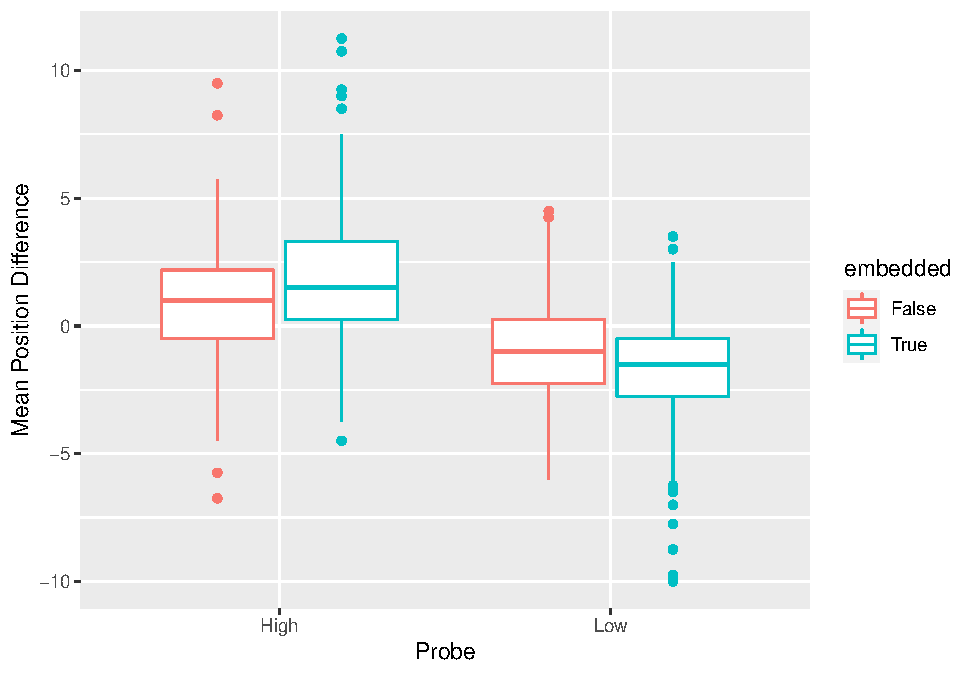
\includegraphics{FinalScientificReport_files/figure-latex/GGPlotBoxplot-1.pdf}
\caption{\label{fig:GGPlotBoxplot}Boxplot of speech perception differences between words and vowels}
\end{figure}



\begin{figure}
\centering
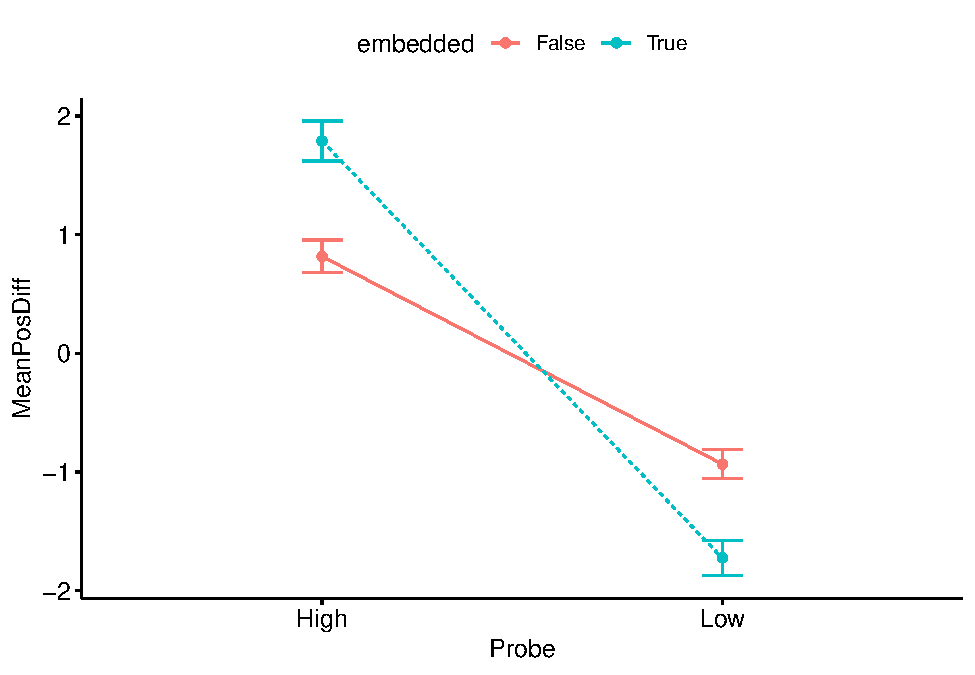
\includegraphics{FinalScientificReport_files/figure-latex/GGPlotLine-1.pdf}
\caption{\label{fig:GGPlotLine}Difference in context effects for words and vowels}
\end{figure}



\begin{figure}
\centering
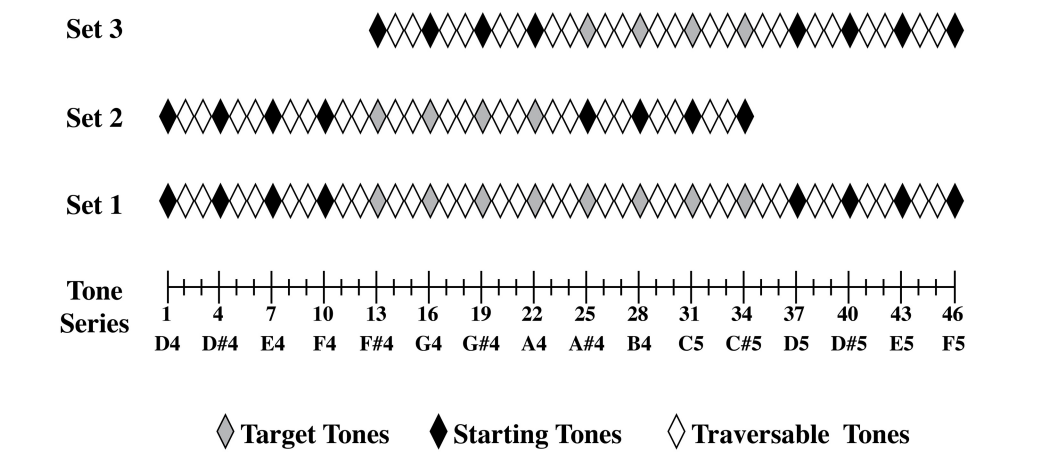
\includegraphics{tones.png}
\caption{\label{fig:fig-tonescale}Diagram of the range of tones used for the probe and target tones}
\end{figure}

\begin{table}[tbp]

\begin{center}
\begin{threeparttable}

\caption{\label{tab:table-MeanPosDiff}Overall Bias in Correct Tone Position Selection for Subjects}

\begin{tabular}{ll}
\toprule
Subject & \multicolumn{1}{c}{mean.MeanPosDiff}\\
\midrule
1 & 0.10\\
2 & -0.37\\
3 & -0.60\\
4 & 0.58\\
5 & -0.27\\
6 & 0.13\\
7 & 0.56\\
8 & 0.18\\
9 & 0.17\\
10 & -0.17\\
11 & -0.08\\
12 & 0.27\\
13 & 0.03\\
14 & 0.66\\
15 & -0.40\\
16 & 0.32\\
17 & -0.47\\
18 & -0.20\\
19 & -0.55\\
20 & -0.99\\
\bottomrule
\end{tabular}

\end{threeparttable}
\end{center}

\end{table}



\hypertarget{references}{%
\section{References}\label{references}}

\hypertarget{refs}{}
\begin{CSLReferences}{1}{0}
\leavevmode\vadjust pre{\hypertarget{ref-deSaussure:19161959}{}}%
Ferdinand de Saussure. (1959/1916). \emph{A course in general linguistics}. McGraw-Hill.

\leavevmode\vadjust pre{\hypertarget{ref-appelbaum:1996}{}}%
Irene Appelbaum. (1996). \emph{The lack of invariance problem and the goal of speech perception}. Retrieved from \url{https://ieeexplore.ieee.org/abstract/document/607912}

\leavevmode\vadjust pre{\hypertarget{ref-posner:1968}{}}%
Michael I. Posner, Steven W. Keele. (1968). \emph{On the genesis of abstract ideas}. Retrieved from \url{https://doi.org/10.1037/h0025953}

\leavevmode\vadjust pre{\hypertarget{ref-robertgoldstone1996}{}}%
Robert Goldstone. (1996). \emph{Isolated and interrelated concepts}. Retrieved from \url{https://doi.org/10.3758/BF03201087}

\leavevmode\vadjust pre{\hypertarget{ref-heald:2014}{}}%
Shannon L.M. Heald, Stephen C. Van Hedger, Howard C. Nusbaum. (2014). \emph{Auditory category knowledge in experts and novices}. \emph{8}. Retrieved from \url{https://doi.org/10.3389/fnins.2014.00260}

\end{CSLReferences}


\end{document}
